\section{The Large Hadron Collider}
\label{sec:LHC}

\subsection{A brief history of the LHC and CMS}
\label{ssec:LHCHist}
% TODO move ref
All dates from the LHC timeline are taken from\,\cite{LHCtimeline}.
The first public announcement of the construction of the LHC was approved on the 16th December 1994. 
A couple of years earlier, on the 1st October 1992, the CMS experiment submitted its letter of intent to the LHC Experiments Committee and on the 31st January 1997, the CMS experiment was approved.
Construction of the CMS site at Cessy began in July 1998, with the complete CMS cavern being inaugerated on the 1st February 2005.
In the following three years, the detector was assembled at the surface in slices and lowered down into the cavern with the final large detector piece being lowered on the 23rd July 2008.
The final dipole magnet of the LHC was lowered into place on 26 April 2007, heralding the completion of the full accelerator ring.
The 10th September 2008, was a very significant day in the history of the LHC marking the first circulation of proton beams around the collider. 
Shortly after, on the 19th, a fault occured in an electrical connection between a dipole and quadrupole magnet, leading to a release of Helium in the tunnels, causing significant damage to the LHC. 
In total 37 damaged magnets were replaced and 16 refurbished, with the final one being lowered on the 30th April 2009. 
Beams were present again in the machine on the 20th November, over a year after the malfunction. 

Run I physics data collection at a centre-of-mass energy, $\sqrts=7\TeV$, was started on the 30th March 2010 and ran through until the 18th October. 
A second period of data collection at $\sqrts=8\TeV$ was performed from the 5th April 2012 to the 6th February 2013. 
During this time, enough data was collected to confirm the existence of a SM-like \Hboson{} boson, officially announced on the 4th July 2012.
With one of the primary mandates of the LHC fulfilled, attention has turned to discovering the existence of physics beyond the SM and measuring precisely the properties of the \Hboson{} and other SM particles.

On the 3rd June 2015, after a 2 year long shutdown for upgrades, the collider started up again for Run II at an unprecendented $\sqrt{s}=13\TeV$. 
Four sets of data are scheduled to be taken during Run II, with a small set taken at the end of 2015 and major runs during 2016, 2017 and 2018.
Each major run lasts from a commissioning period around March to the end-of-year techinical stop in December.
Run II data is scheduled to be collected until December 2018, from when it will enter a second long shutdown period.
This thesis uses the data set collected during 2016.

\subsection{Operating the LHC}
\label{ssec:LHCoperation}

The source for the proton beams is a small canister of hydrogen gas. 
The hydrogen gas is then ionised to create protons by applying a large electric field.
The collection of protons is then accelerated, within ultra-high vacuums, through the Linear Accelerator 2 (LINAC2), which uses alternatingly charged conductors to both pull and push the bunch of protons up to an $\sqrt{s}=50\MeV$, before being injected into the Proton Synchrotron Booster (PSB).
The PSB is an accelerator ring that boosts the protons to $\sqrt{s}=1.4\GeV$ and passes them to the Proton Synchrotron (PS) which provides a further boost to $\sqrt{s}=25\GeV$.
From the PS the proton bunches are accelerated in the Super Proton Synchrotron (SPS) to $\sqrt{s}=450\GeV$. 
The SPS splits the single beam into two counter-rotating ones and injects them into the LHC.
In the LHC, each proton beam can be accelerated up to a maximum $\sqrt{s}=7\TeV$ per beam. 
During Run I, this beam energy was operated at $\sqrt{s}=3.5(4)\TeV$ and has been increased to $\sqrt{s}=6.5\TeV$ for Run II. 
The full accelerator complex at CERN is shown in Fig.\,\ref{fig:CERNcomplex}.
\begin{figure}[htpb]
	\centering
	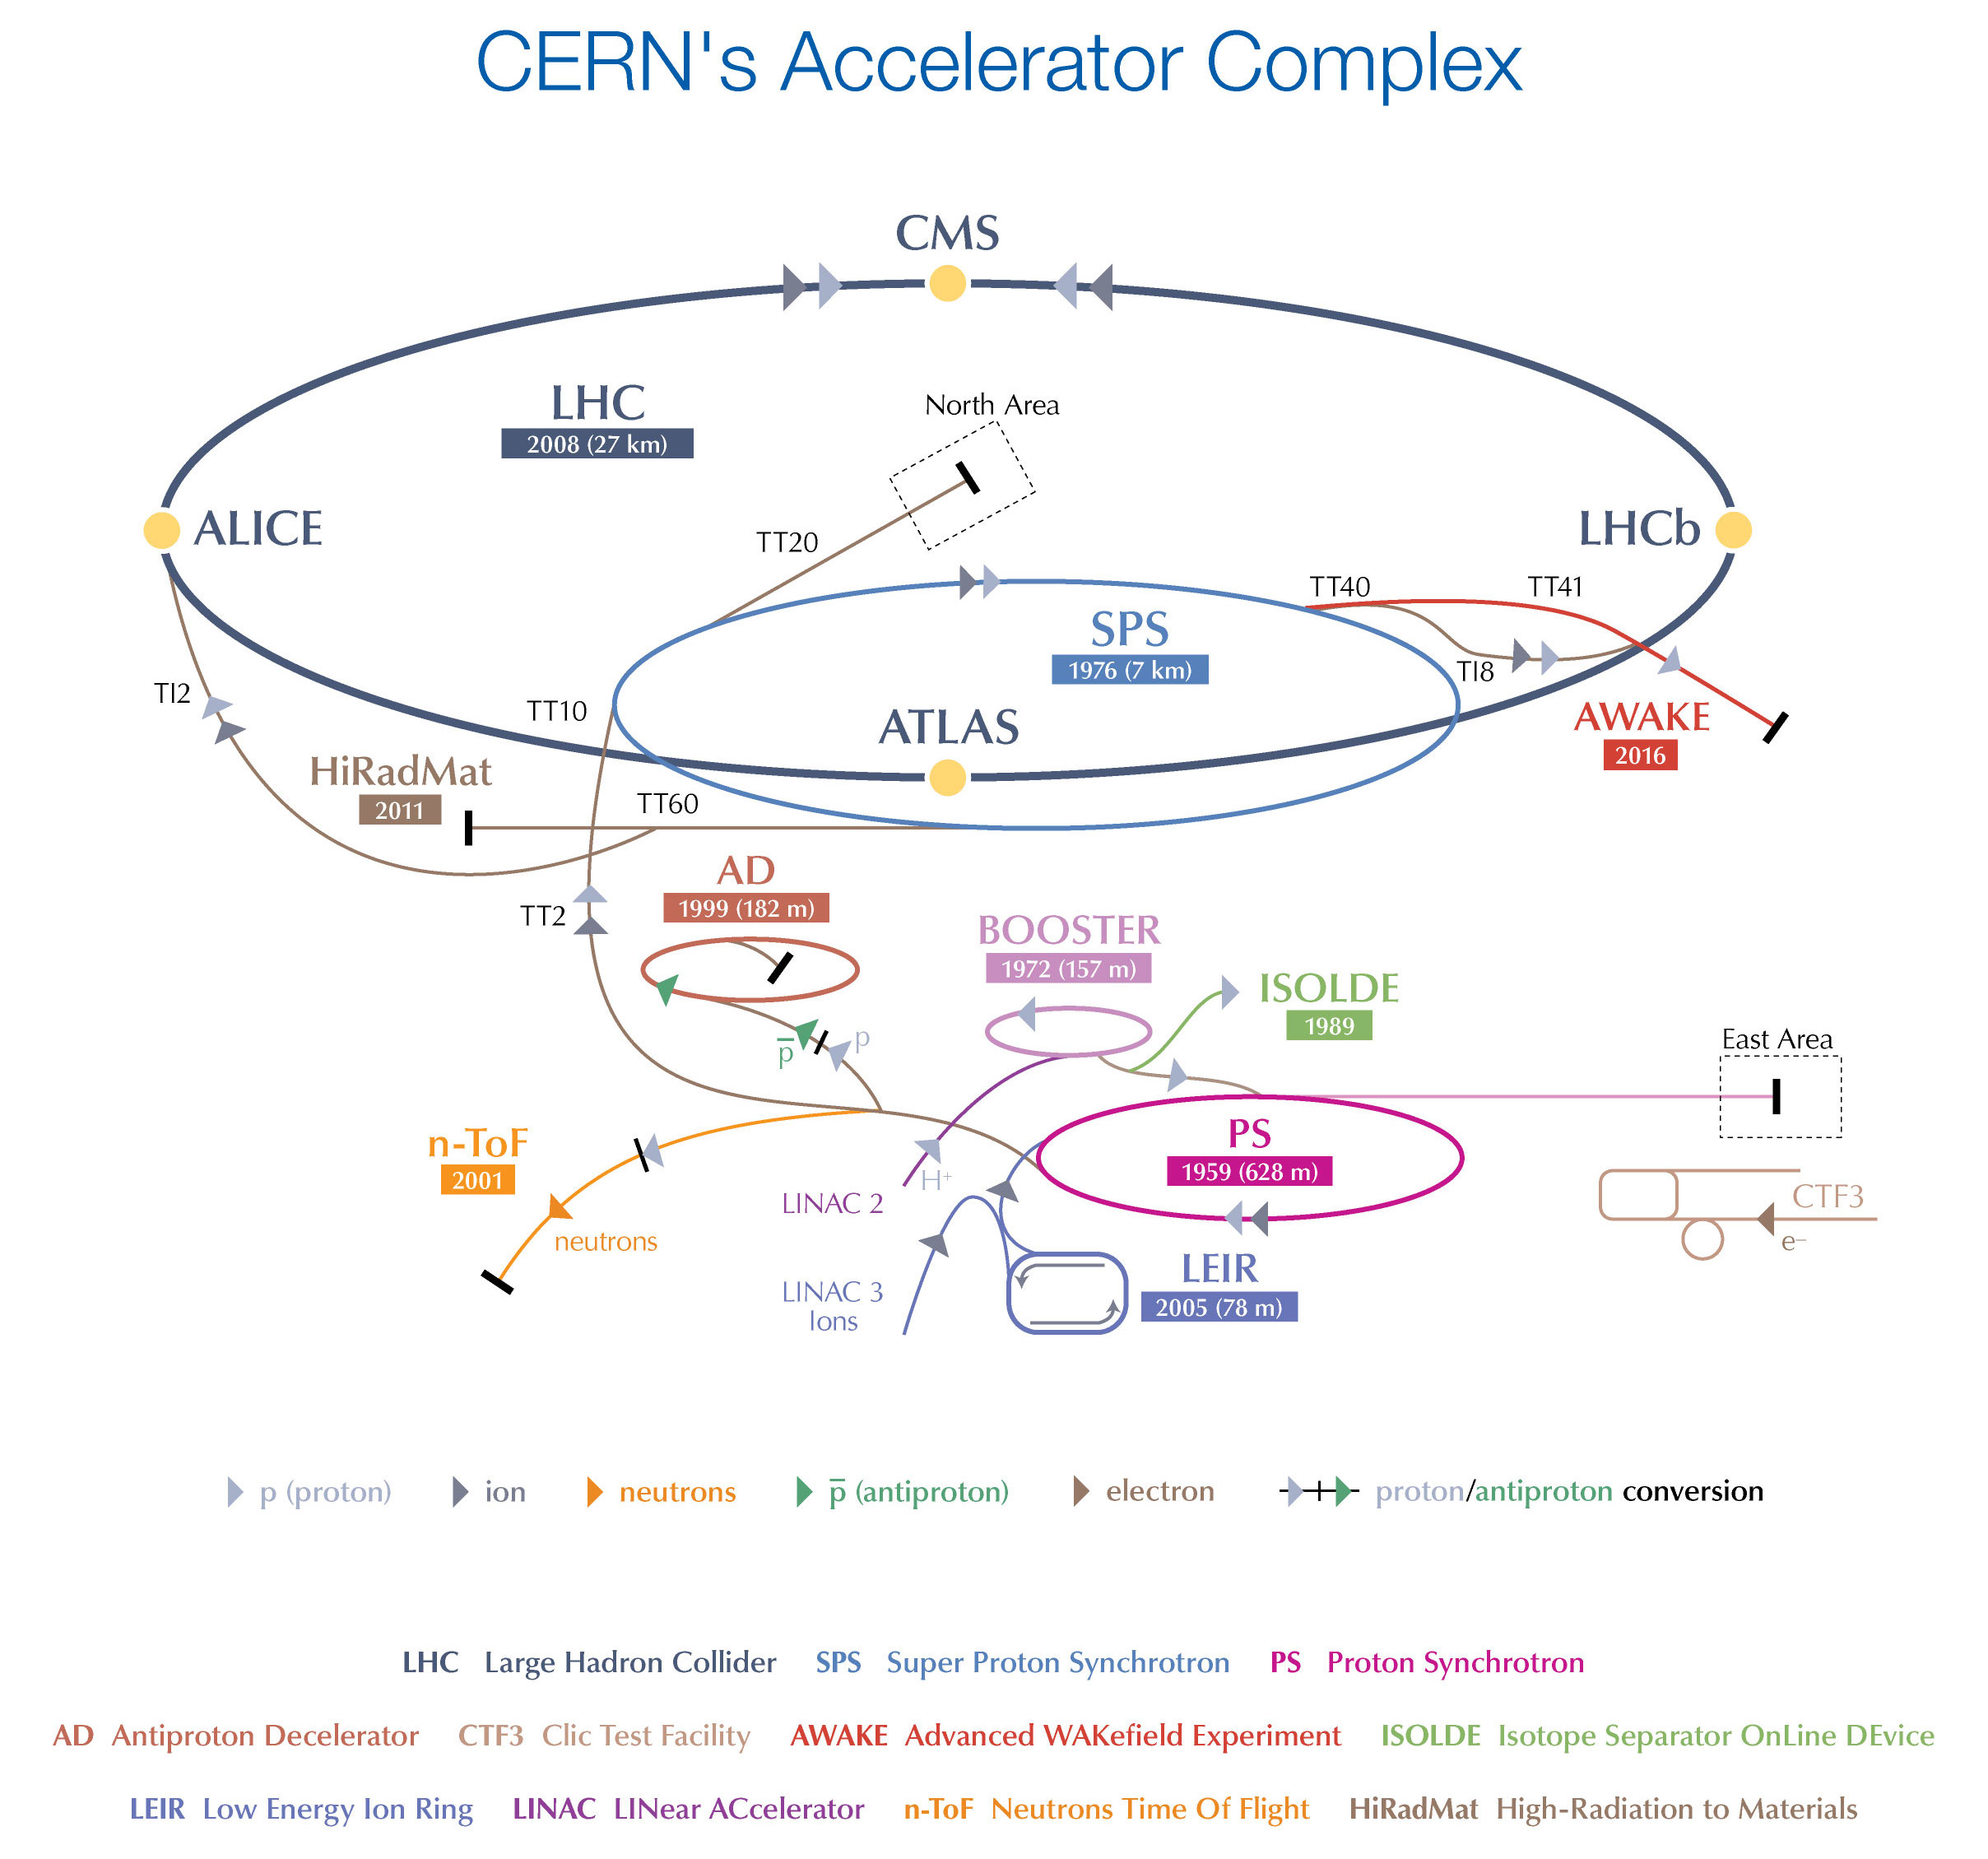
\includegraphics[width=0.8\textwidth, rotate=90]{Figures/CERNcomplex}
	\caption[The full CERN complex showing schematically the location of all the experiments on the ring complex.]{The full CERN complex showing schematically the location of all the experiments on the ring complex.\,\cite{CERNcomplex}. }
	\label{fig:CERNcomplex}
\end{figure}
To reach these operational collision energies the proton bunches are accelerated and confined by magnetic fields of up to 8.3\Tesla{} from over 9300 superconducting magnets. 
% TODO Beam Structure?
% http://public-archive.web.cern.ch/public-archive/en/lhc/Facts-en.html

\subsection{Magnets at the LHC}
\label{ssec:LHCmag}
The LHC uses magnets to accelerate, focus and squeeze the proton beams.
The most common type of magnet used in the LHC is the dipole magnet, of which there are 1232.
Each dipole magnet is 15\m{} long, weighs 35 tonnes and has a magnetic field strenth of 8.3\Tesla{} which is used to accelerate the proton bunches to 6.5\TeV{} and bend the beam around the collider. 
Figure~\ref{fig:LHCdipole} shows a cross section through one of the LHC dipole magnets.
Each dipole contains two beam pipes for the counter-circulating beams and along each of these beam pipes are coiled niobium-titanium alloy wires which form the superconducting dipole magnet. 
Superconductivity in the magnet is acheived by a closed circuit of liquid helium, which cools the iron yoke to 1.9\Kelvin{}.
% Different specs for inner outer coils: http://lss.fnal.gov/archive/2015/conf/fermilab-conf-15-635-td.pdf
\begin{figure}[htpb]
	\centering
	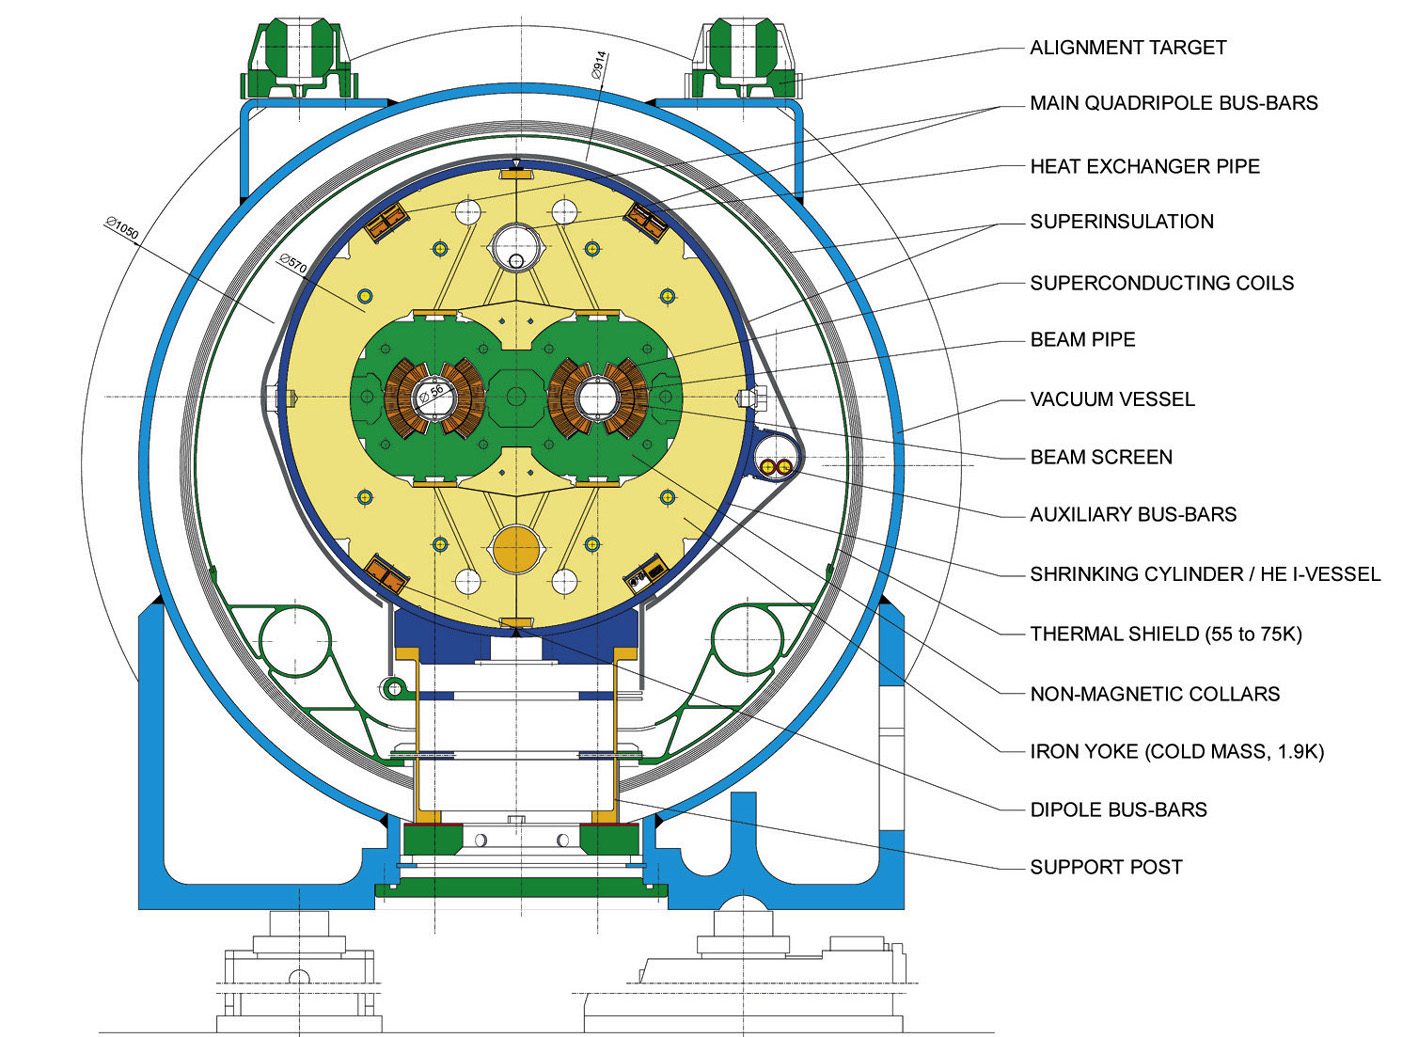
\includegraphics[width=0.9\textwidth]{Figures/LHCdipole}
	\caption[A cross section of a LHC dipole magnet]{A cross section of a LHC dipole magnet \cite{LHCdipolemagnet}. }
	\label{fig:LHCdipole}
\end{figure}
% Busbar = highvoltage power rail

% http://ieeexplore.ieee.org/stamp/stamp.jsp?arnumber=1211818
In addition to the dipole magnets, the LHC uses 858 quadrupole magnets. 
Of these, 392 are lattice quadrupoles used to stop the beam from defocussing over time due to the similarly charged beam constituents. 
Quadrupole magnets are also used to confine the proton beams as they are entering the experimental caverns. A set of three, known as an inner triplet, squeezes each beam to a diameter of 16\um{} to ensure a maximal number of collisions at the interaction point.
Increasing the number of collisions leads to a higher event rate, described by the quantity known as the instantaneous luminosity (\Lum{}). % why is high event rate good?
There are additional multipole magnets used to correct for other, smaller, effects present in the beam, such as the gravitational force on the protons. 
% electromagnetic interactions among bunches, electron clouds from the pipe wall
%TODO check explain and reference.


\subsection{Luminosity measurements}
\label{ssec:lumi}

% \Lum{} gives a good description of the state of the beams
The instantaneous luminosity is defined as:

\begin{equation}
\label{eq:InsLumi}
\Lum = f \frac{n_{1}n_{2}}{4\pi \sigma_{x} \sigma_{y}}
\end{equation}
% sigma^2 (beam size) = epsilon.beta* (emittance . beta function)
% emittance – the spatial and angular spread of particles. A low emittance particle beam is a beam where the particles are confined to a small distance and have nearly the same momentum.

\Lum{} depends on the bunch crossing rate, $f$, the number of protons in each colliding bunch, $n_{1}$ and $n_{2}$, and the root-mean-square of the transverse beam sizes in the horizontal ($\sigma_{x}$) and vertical ($\sigma_{y}$) directions. 
The beams are assumed to have a gaussian profile, of width $\sigma=16\um$, and to be colliding head-on.
% Not head on add another crossing angle factor
% Is this true? Probably not
For nominal running during Run II, each beam contains 3564 bunch spaces of which typically 2808 are filled during data taking, leading to a minimum bunch spacing of 25\ns{} and a collision rate $f=40\MHz$.
% TODO find reference
Each bunch contains $\approx 1.1\ten{11}$ protons, producing a peak $\Lum=1.50\ten{34}\Lunit$.
\Lum{} varies with respect to time due to the depletion of the protons in each bunch after every collision.
TODO: REDUCED SIGMAX AND SIGMAY DUE TO REDUCED NPROTON?
% 1.15 is design, 1.1 is actual http://accelconf.web.cern.ch/accelconf/hb2016/papers/moam5p50.pdf
% 27km / 3564b / 3e8 = 25ns :D
% Check

The total number of collisions produced at the LHC, in a time $t$, can be estimated from the luminosity by:
\begin{equation}
\label{eq:nEvent}
\text{N} = \sigma_{\text{minbias}} \times \Lum_{\text{int}}, 
\end{equation}
where $\sigma_{\text{minbias}}$ is the minimum bias cross section and $\Lum_{\text{int}}$, is the integrated instantaneous luminosity over time $t$:
\begin{equation}
\label{eq:IntLumi}
\Lum_{\text{int}} = \int^{t}_{t_{0}}\Lum(t) dt
\end{equation}
The peak \Lum{} and $\Lum_{\text{int}}$ distributions during the 2016 data taking period are shown in the left and right panels of Fig.~\ref{fig:CMSLumi} respectively.
A total of \Lumi{} of certified data was collected by CMS during 2016.
Using the current $\sigma_{\text{minbias}}$ measurement of 69.2\mb{}, this means that approximately $2.5\ten{15}$ collisions were processed in this period.

\begin{figure}[htpb!]
	\centering
	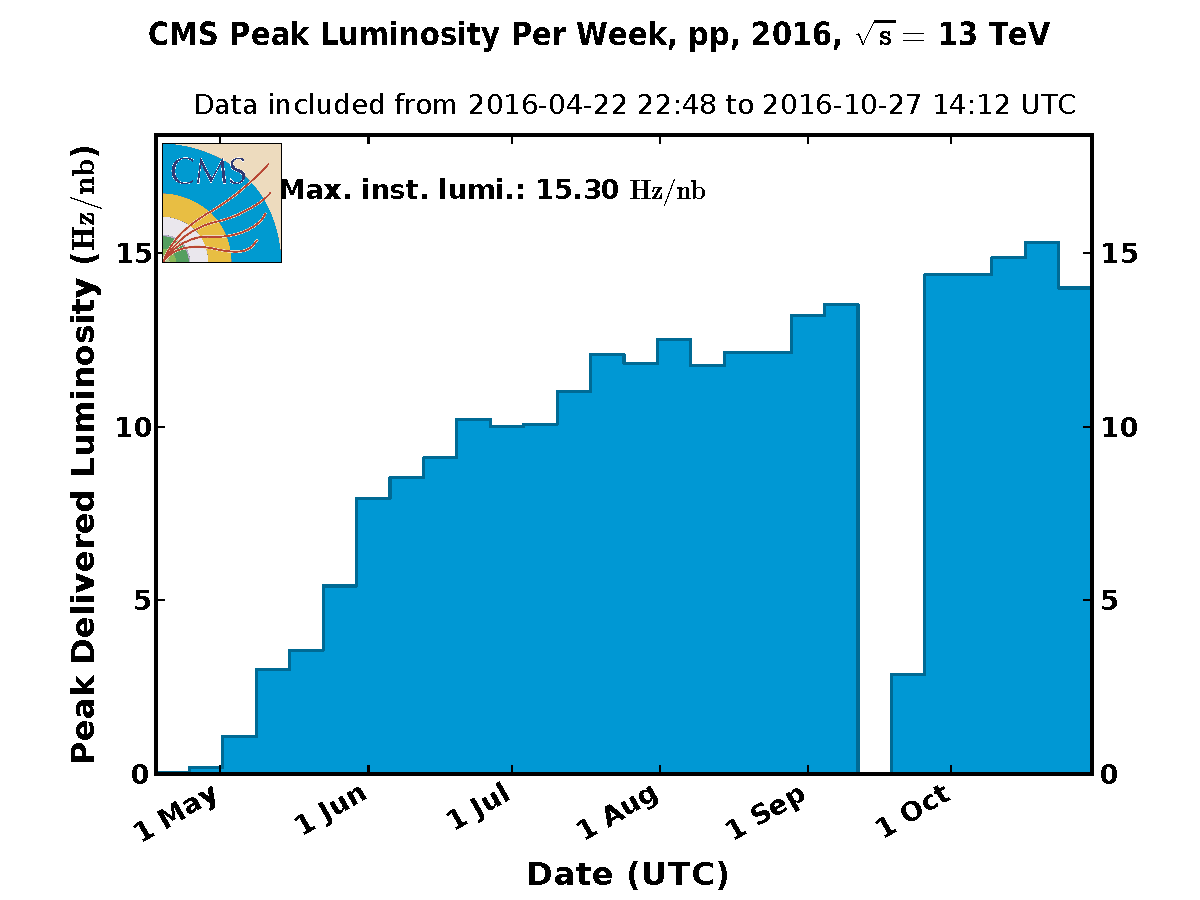
\includegraphics[width=0.49\textwidth]{Figures/CMS2016PeakLumi}
	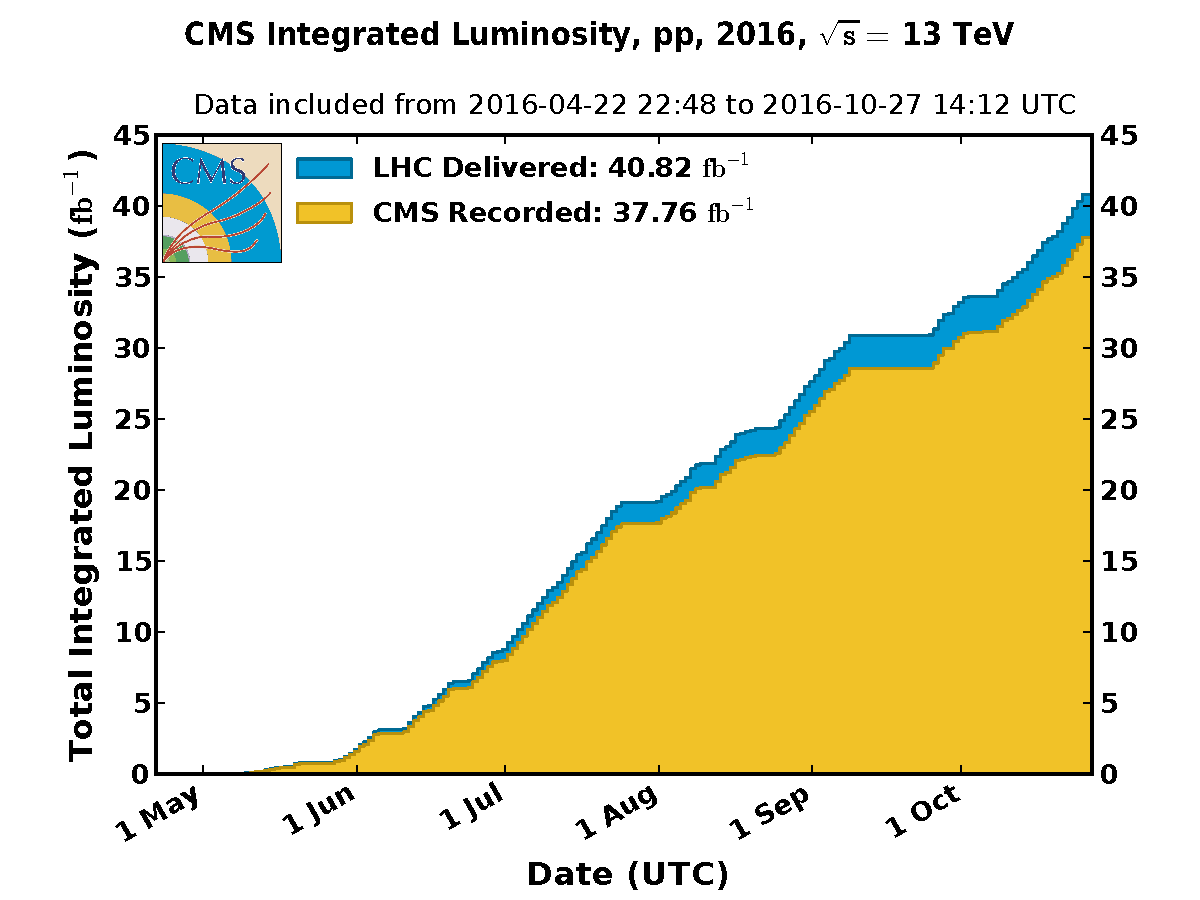
\includegraphics[width=0.49\textwidth]{Figures/LHC2016Lumi}
	\caption[The left panel shows the peak luminosity produced per week of running during 2016. The right panel shows the integrated luminosity that the LHC delivered and CMS recorded during the same period of time.]{The left panel shows the peak luminosity produced per week of running during 2016. The right panel shows the integrated luminosity that the LHC delivered and that the CMS experiment recorded during the same period of time. }
	\label{fig:CMSLumi}
\end{figure}

In every bunch crossing, more than one proton-proton collision occurs.
These additional interactions are collectively known as pileup.
Pileup cannot be directly measured, but can be inferred from the number of reconstructed vertices in the event.
It can have a significant effect on the kinematical properties of any jets produced by contributing particles from its interaction to the jet clustering algorithms centered on the primary vertex.
The distribution of pileup seen at CMS during 2016, shown in Fig.~\ref{fig:CMSPU}, has an average of $\approx30$ additional interactions for every hard interaction.
Methods of pileup mitigation are explained later in Section TODO.
% Link to Tracker - lots of particles need high granularity tracker.
\begin{figure}[htpb]
	\centering
	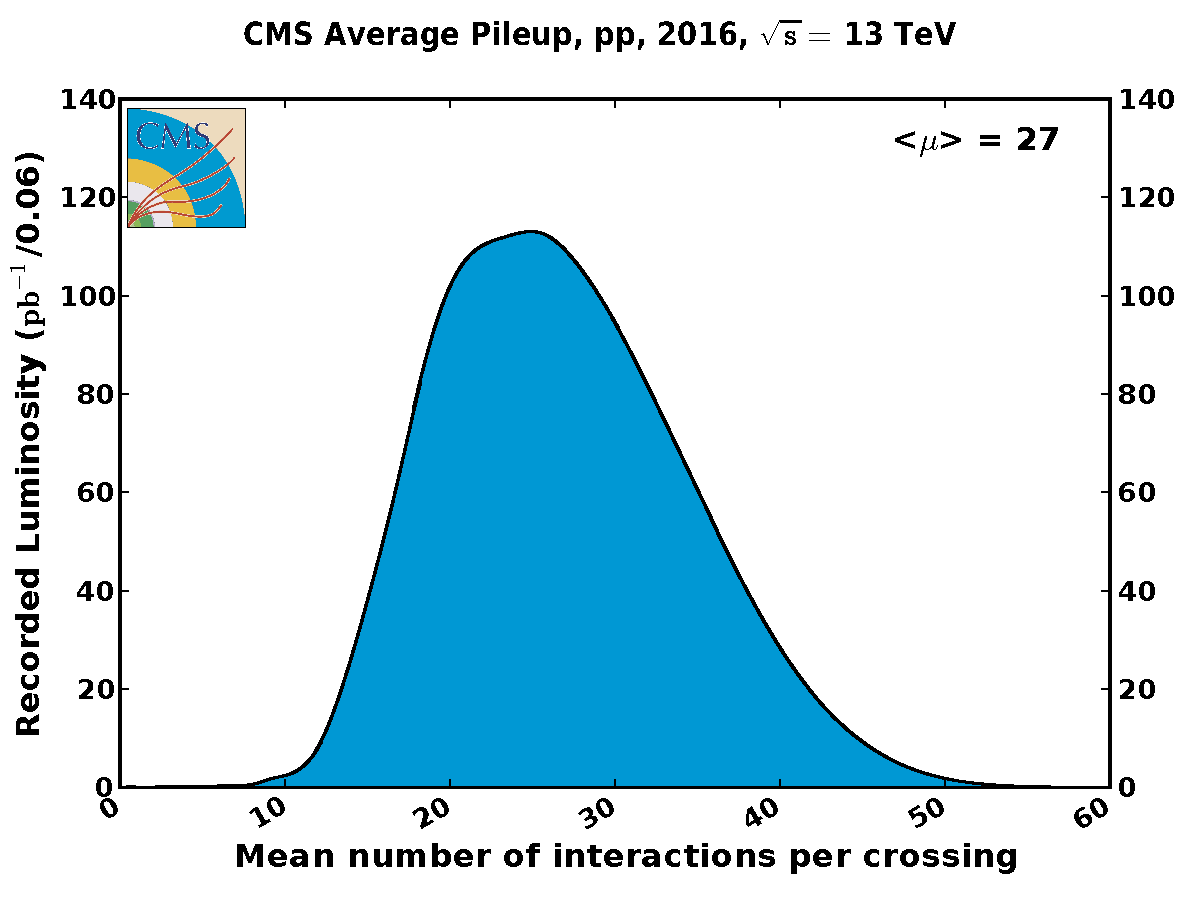
\includegraphics[width=0.5\textwidth]{Figures/CMSAvePU}
	\caption[The distribution of the number of interactions in bunch crossing]{The distribution of the number of interactions in bunch crossing. TODO CITE }
	\label{fig:CMSPU}
\end{figure}

To operate in a high luminosity environment, the CMS experiment must have excellent resolution in each of its measuring instruments, combined with a low latency due to the high collision rate. 
The materials used must be reliable, while having maximal longevity when operating in a high-radiation environment.